\section{A Framework for Holistic Co-Design}\label{sec:apx:holisticcodesign:holistic_co_design_framework}
\begin{figure}[h!]
    \centering
    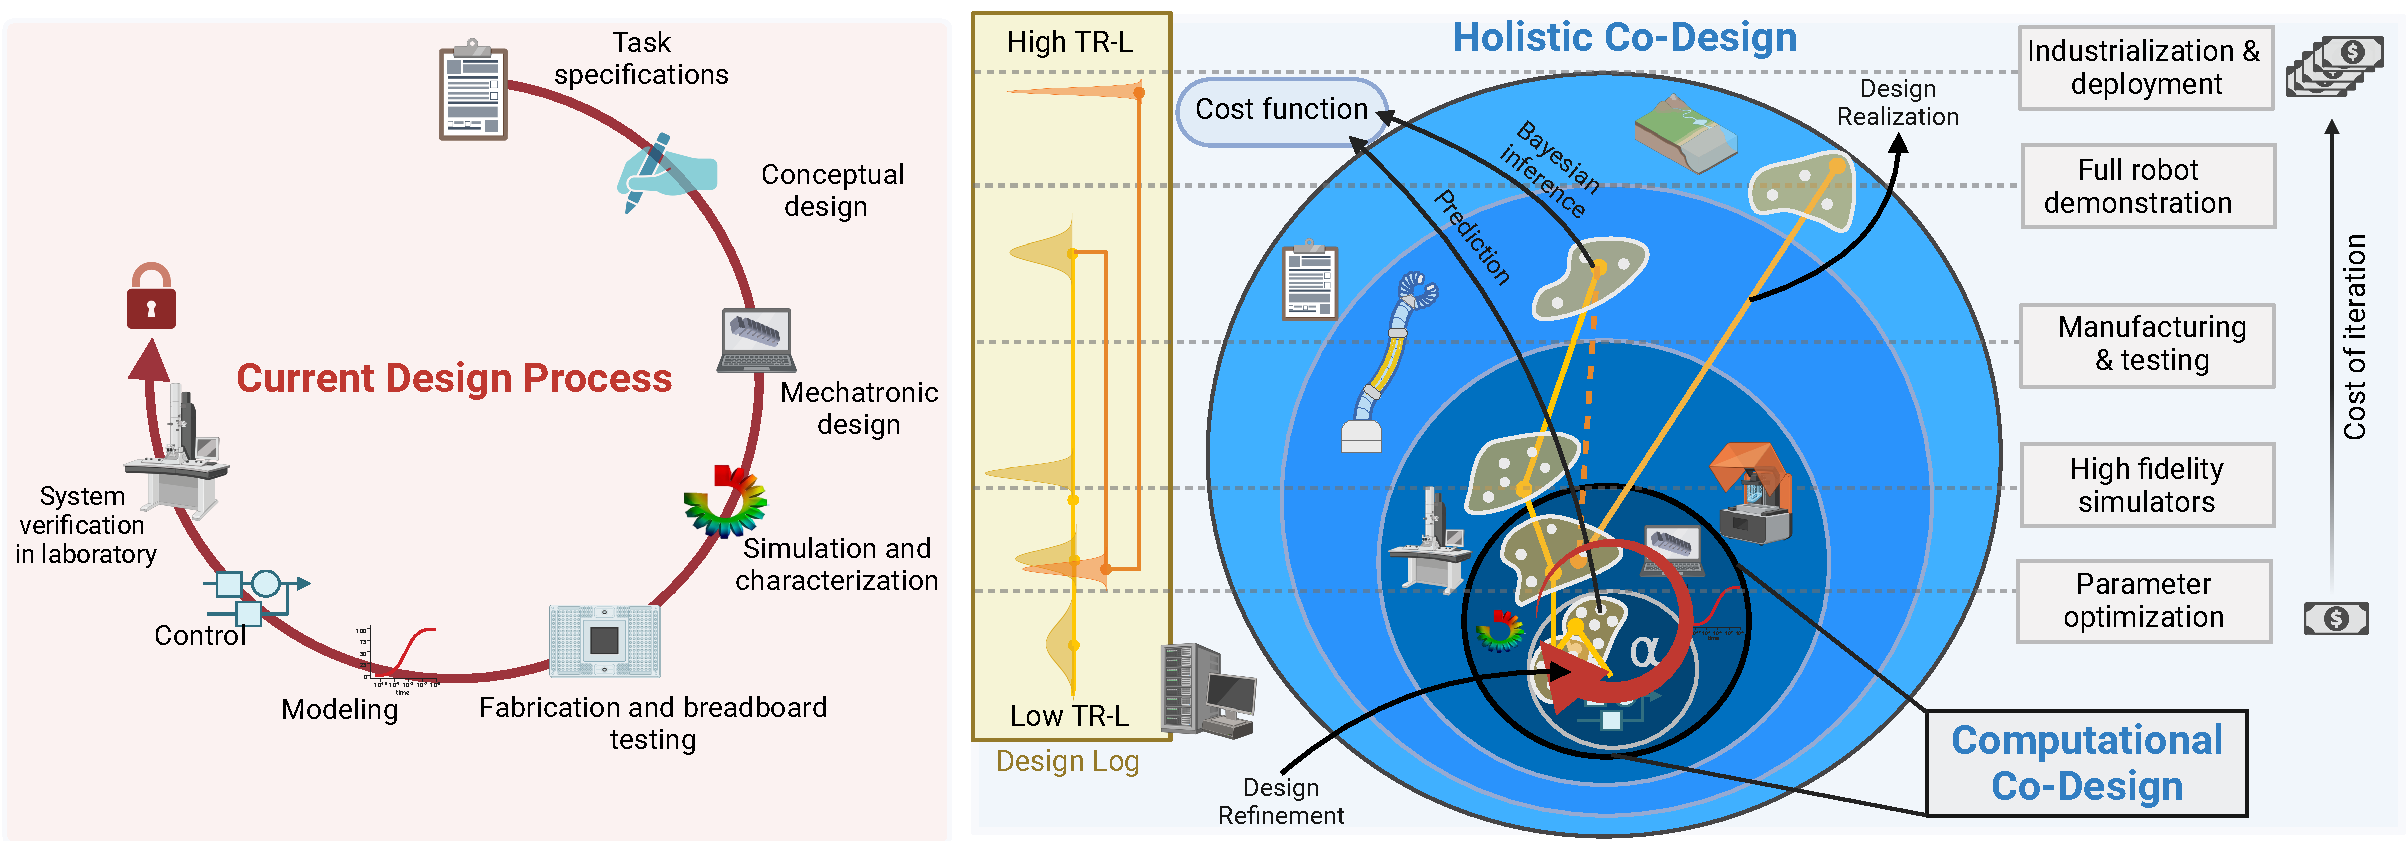
\includegraphics[width=1\linewidth]{appendix-holistic-codesign/figures/current_design_vs_holistic_codesign_v1.pdf}
    \caption{
        \textbf{Left:} A basic design cycle applied to soft robots, which mirrors how soft robots have been traditionally developed. It follows a very sequential approach and lacks feedback loops to iteratively and efficiently improve the design.
        \textbf{Right:} The holistic design contains different layers where the design is co-optimized, considering the cost of a new analysis and the relative reduction in uncertainty associated.
    }
    \label{fig:apx:holisticcodesign:current_design_vs_holistic_codesign}
\end{figure}

Holistic co-design marks a significant shift in soft robotics by adopting an integrated, application-driven strategy that emphasizes the seamless interaction between a robot’s physical morphology, its control system, and user engagement. Unlike traditional design cycles—which remain prevalent—it provides a structured framework that concurrently develops all system components, refining the design iteratively through effective feedback loops. Moreover, this approach distinguishes itself from other co-design methods by embracing a broader set of design values, advocating for cross-disciplinary collaboration and active participation from diverse stakeholders, introducing techniques to enhance computational efficiency, and proposing a probabilistic view that acknowledges uncertainties in evaluation metrics while outlining strategies to mitigate them as the design evolves.

In detail, the proposed holistic co-design framework introduces several key innovations. First, it optimizes a range of design attributes simultaneously—such as task completion time, safety, material and fabrication costs, energy consumption, and environmental impact—instead of focusing on a single metric like locomotion speed, as most current approaches do. Second, it significantly boosts the efficiency of computational co-design by (i) establishing a reduced-order design space that avoids the complexity of directly optimizing a high-dimensional spatial morphology (as seen in voxel-based methods); (ii) developing a control-oriented reduced-order model within the co-design process; (iii) employing computationally inexpensive auxiliary metrics, such as controllability, observability (leveraging the reduced-order model), or manufacturability, which provide early feedback to the optimizer instead of relying solely on the outcome of resource-intensive closed-loop simulations; and (iv) efficient derivation/learning of controllers based on the reduced-order model (i.e., model-based control).
Furthermore, while existing methods typically address only the fully computational aspects of design and evaluation, our framework explicitly accounts for the inherent uncertainties in these metrics—uncertainties that can only be properly identified through high-fidelity simulations or, ideally, extensive testing with physical prototypes. By introducing a probabilistic evaluation of a design’s “fitness,” we also formalize strategies to reduce such uncertainties through prototyping, as visualized in Fig.~\ref{fig:apx:holisticcodesign:current_design_vs_holistic_codesign}~(Right). Additionally, we emphasize that collaboration among team members with varied expertise and backgrounds, as well as engagement with stakeholders (including customers, scientific advisors, and domain experts), is essential for developing a high-performing soft robot. Finally, we conclude that co-design approaches not only help preserve design knowledge but also enhance reproducibility, addressing a well-known challenge in soft robotics~\citep{baines2024need}.

\paragraph{Multi-Objective Co-Design: Satisfying Comprehensive Requirements and Evaluation Metrics}
Current co-design approaches for soft robots typically consider only one, or at most a few, evaluation metrics\footnote{Commonly, such evaluation metrics are also referred to as costs, losses, or rewards} per task~\citep{spielberg2019learning, spielberg2021co, medvet2022impact, wang2023preco, wang2024diffusebot, navez2024design}. For locomotion tasks, this often means measuring the velocity achieved or the distance traveled in a fixed time period~\citep{spielberg2019learning, wang2023preco}, while in manipulation tasks (e.g., pushing), the focus is on how far an object is safely moved~\citep{wang2024diffusebot}. However, as soft robots evolve from research prototypes into commercial products, a broader set of design values becomes critical. These include, but are not limited to, safety (as discussed in Chapter~\ref{chp:safetymetric}), manufacturing costs (especially in relation to production batch sizes)~\citep{miriyev2017soft, schmitt2018soft, majidi2014soft, junge2022leveraging}, material supply, and the robot’s operational lifetime—which depends on both the materials used and the stresses experienced—as well as ecological and recycling considerations~\citep{mazzolai2020vision}. Additionally, regulatory requirements grow in significance; traditional design processes tend to address regulatory standards only at the end or not at all, whereas regulatory compliance is essential from the start. For example, medical soft robots must meet the FDA or EMA guidelines, which dictate acceptable materials, manufacturing methods, and performance criteria. Incorporating these regulatory factors into the design optimization loop helps prevent late-stage redesigns that could delay product deployment and significantly increase development costs. Holistic co-design integrates these values and constraints from the beginning, ensuring that the resulting designs are optimal across all dimensions.

\paragraph{Increasing the Efficiency of Computational Co-Design}
\emph{Computational co-design} for soft robots refers to developing an automatic algorithm that optimizes the integrated design (encompassing both body and control components) to meet specified performance criteria and design values~\citep{carlone2019robot, wang2023softzoo}. In its most general form, co-design can be formulated as a constrained nonlinear optimization problem~\citep{zardini2023co} over a parameterized design $x$, such that
\begin{equation}
\begin{aligned}
    \min_{x} \quad & f(x)\\
    \textrm{s.t.} \quad & g(x) = 0 \\
    & h(x) \leq 0,
\end{aligned}
\end{equation}
where $f(x): \mathcal{X} \to \mathcal{C}$ represents the cost or loss function, and $g(x): \mathcal{X} \to \mathbb{R}^{n_\mathrm{eq}}$ and $h(x): \mathcal{X} \to \mathbb{R}^{n_\mathrm{ineq}}$ denote the equality and inequality constraints, respectively. For example, in multi-objective optimization, we can define $f(x) = \begin{bmatrix} \hat{c}_1^\top(x), \dots, \hat{c}_{n_\mathrm{obj}}^\top(x) \end{bmatrix}^\top$, with each $f_j(x) = \hat{c}_j(x)$ for $j = 1, \dots, n_\mathrm{obj}$ corresponding to design objectives implemented via the (estimated) evaluation metrics $\hat{c}_j(x): \mathcal{X} \to \mathcal{C}_j$. These objectives might include task performance, manufacturing, and operational costs, or environmental impact. Equality constraints typically capture system dynamics, while inequality constraints ensure physical feasibility (such as non-negative volume, adherence to manufacturing tolerances, or minimum geometric dimensions for manufacturability) and guarantee that the design satisfies essential requirements (like minimum safety levels or regulatory standards). Please note that such (inequality) constraints can also be a function of an estimated evaluation metric $\hat{c}_j(x)$.

In our view, one key reason co-design approaches are not yet widely adopted in soft robotics is their computational inefficiency and high cost, which severely restrict the design space that can be explored and diminish the chances of finding the optimal design, thereby reducing their practical utility~\citep{chen2020design}. We identify three primary sources of computational inefficiency in current methods: (i) they often operate in high-dimensional design spaces—for instance, by discretizing the soft robotic geometry into voxels—which makes it extremely challenging, if not impossible, to locate the global optimum; (ii) the optimization loop is closed via performance metrics obtained from one or multiple closed-loop system simulations, and using high-fidelity simulators makes this evaluation process computationally demanding; (iii) assessing closed-loop performance requires access to a controller. In principle, there are two ways to address this: one can train a controller over a set of different designs~\citep{zardini2021seeking, boekel2025learning}, though this means the controller may not be optimized for a specific design, so the evaluation might not reflect the true performance achievable with a specialized controller. Alternatively, training a controller tailored to the proposed design can fully exploit its kinematics and dynamics to achieve optimal task performance, but this approach is computationally very intensive—especially when using \gls{RL} controllers trained from scratch~\citep{bhatia2021evolution, wang2022curriculum, wang2023softzoo, wang2023preco} or control policies trained via gradient descent using a differentiable simulation~\citep{spielberg2019learning, wang2023softzoo, wang2024diffusebot}—which often struggle with complex hybrid dynamics such as contact.

Our framework, depicted in Fig.~\ref{fig:apx:holisticcodesign:computational_co_design}, paves the way for significantly more efficient computational co-design of soft robots by introducing four key modifications that address the previously mentioned challenges:
% 
(1) Building on previous work~\citep{spielberg2019learning, wang2024diffusebot}, we advocate for performing optimization in a reduced-order design space, which can be either entirely learned or partially defined manually (e.g., specifying the length and diameter of a soft segment). In practice, reduced-order designs $x$ are sampled from a distribution, and then a design decoder reconstructs the full design description (such as a volumetric mesh with sensor and actuator placement). After evaluating the design, the optimizer updates the posterior belief of the sampling distribution to bias it towards effective designs. We elaborate on reduced-order design in Section~\ref{sec:apx:holisticcodesign:reduced_order_design_parametrizations}.
% 
(2) A control-oriented reduced-order model can greatly assist in analyzing the system’s motion characteristics and behavior~\citep{bruder2020data, armanini2023soft, menager2023direct, alora2023data, stolzle2024input, alkayas2025soft, valadas2025learning}. While deriving such models for rigid manipulators is generally straightforward~\citep{siciliano2010robotics, zhao2020robogrammar}, soft robotics presents an inherent interplay between design, actuation, and task (e.g., payload, gravitational forces) on one side and the resulting deformations on the other. This interdependence makes it essential to jointly synthesize the design (including actuation) and the kinematic model. We discuss this further in Sec.~\ref{sec:apx:holisticcodesign:codesigning_physical_intelligence}.
% 
(3) To reduce the reliance on performance metrics derived from resource-intensive closed-loop simulations, we introduce several auxiliary metrics that are computationally cheaper to evaluate. These metrics provide early feedback to the optimizer, allowing for the early discarding of designs with very low predicted fitness. Examples include metrics assessing observability and controllability based on the reduced-order model (which directly links actuator and sensor placement to the structural design), open-loop compliance~\citep{guan2023trimmed}, safety (as discussed in Chapter.~\ref{chp:safetymetric}), embodied intelligence~\citep{cianchetti2021embodied, mengaldo2022concise, vihmar2023measure}, or heuristics estimating manufacturability. We further discuss controllability and observability metrics in Sec.~\ref{sec:apx:holisticcodesign:codesigning_physical_intelligence}.
%
(4) Finally, we propose leveraging the reduced-order model to derive the control law in a model-based fashion. Recent advancements provide a solid foundation for exploiting dynamical models—whether physics-based or data-driven—for control~\citep{della2023model, laschi2023learning}. For example, using Koopman theory to learn a linear model (or linearizing a nonlinear model around equilibrium) enables the design of optimal controllers in closed form via LQR~\citep{bruder2020data}. For nonlinear models with a physical structure (i.e., with well-defined kinetic and potential energy terms)~\citep{armanini2023soft, liu2024physics, stolzle2024input, alkayas2025soft, valadas2025learning}, PID+Feedforward~\citep{della2023model, stolzle2024experimental, stolzle2024input} or similar closed-form controllers (e.g., PD+~\citep{della2020model}, computed torque) can be designed. When dynamics are modeled as generic nonlinear transition functions (e.g., \glspl{RNN}~\citep{thuruthel2017learning}, \glspl{NODE}~\citep{kasaei2023data}), optimal control techniques such as \gls{MPC}~\citep{alora2023data} or model-based \gls{RL}~\citep{thuruthel2018model} can compute the control input. These model-based approaches to deriving a control law are dramatically more computationally efficient than training an \gls{RL} control policy from scratch for each design~\citep{bhatia2021evolution, wang2022curriculum, wang2023softzoo, wang2023preco}.

\begin{figure}[h!]
    \centering
    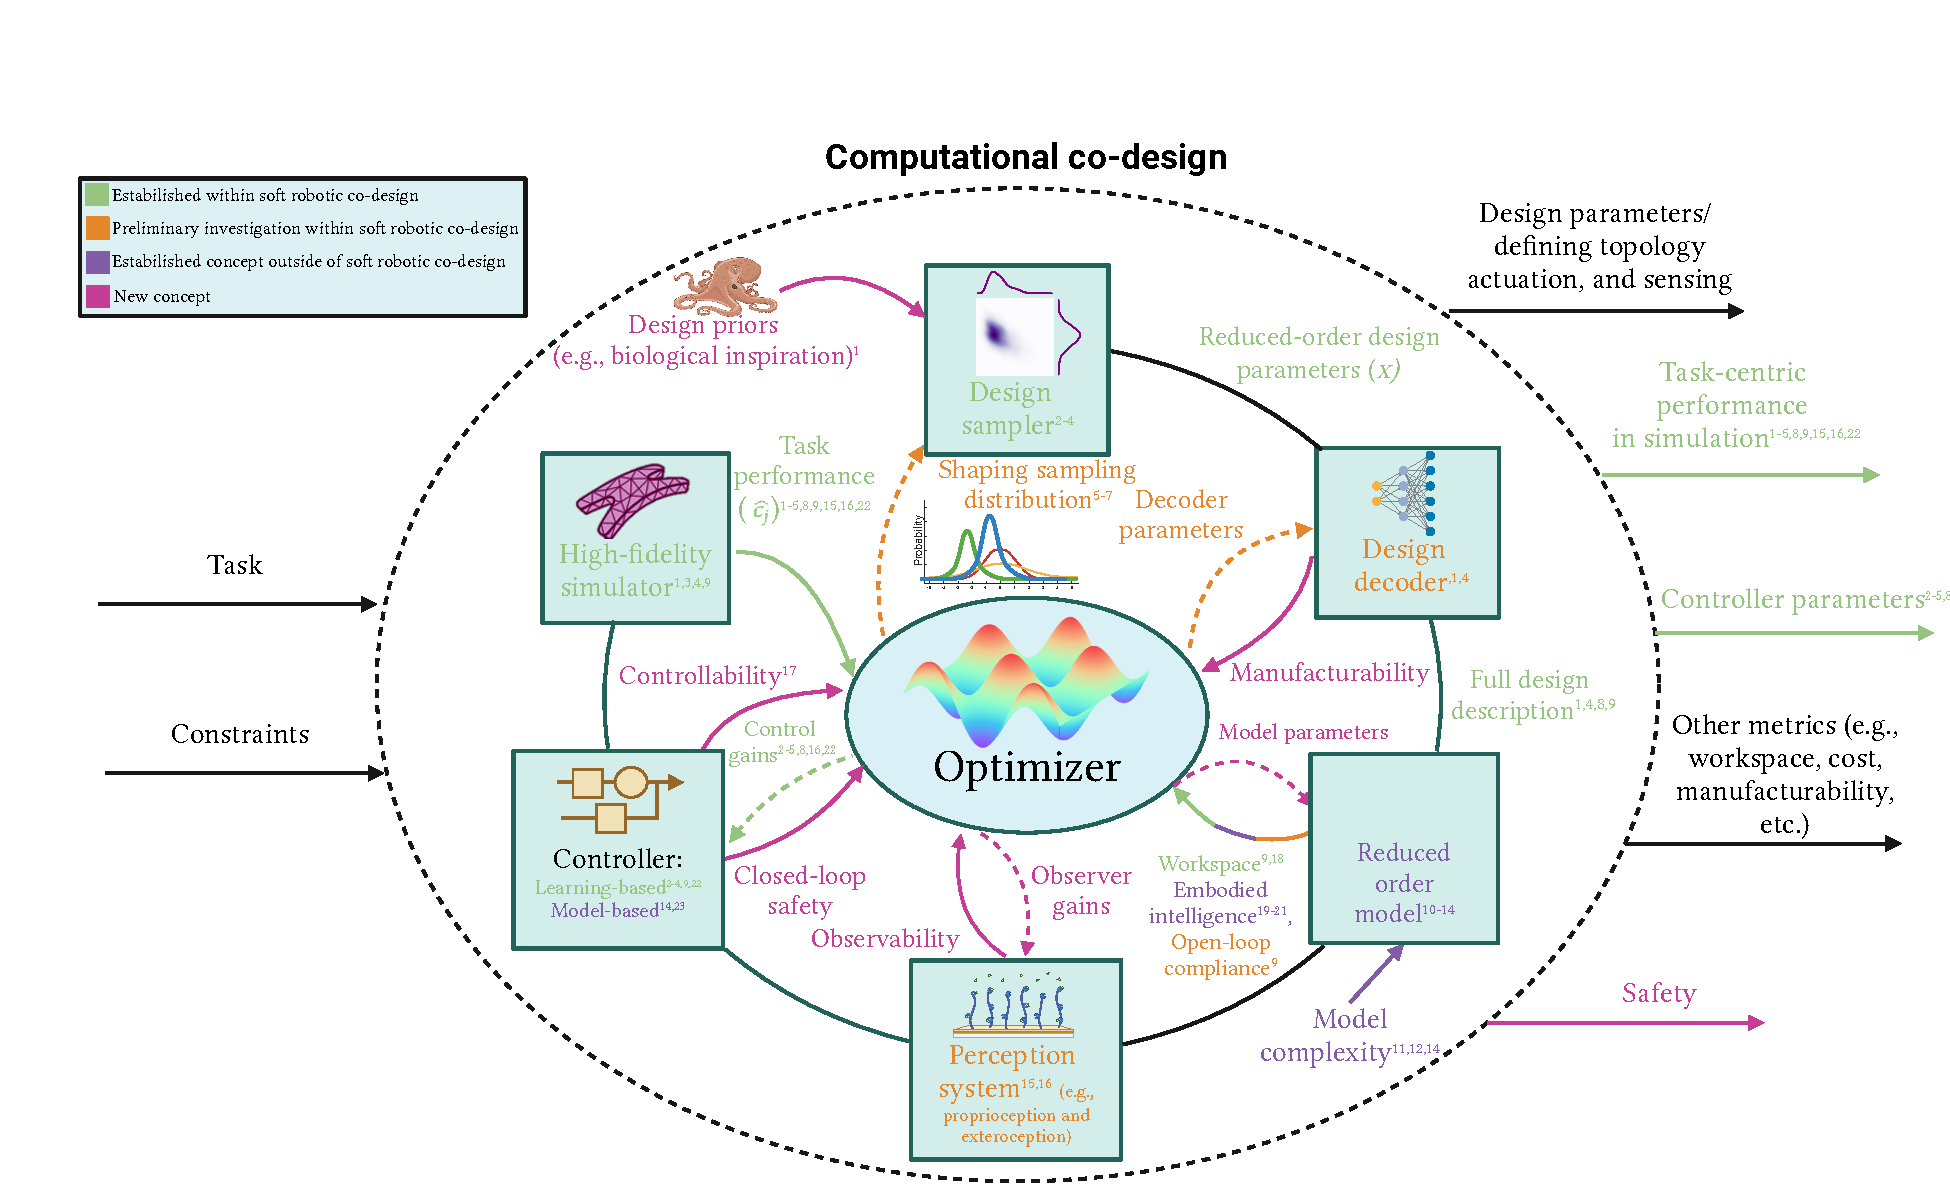
\includegraphics[width=1\linewidth]{appendix-holistic-codesign/figures/computational_codesign_v1.pdf}
    \caption{\textbf{A Framework for Efficient Computational Co-Design of Soft Robots:}
        We sample reduced-order design parameters $x$ from an initial distribution, which can incorporate design priors from biological inspiration~\citep{mazzolai2020vision, chen2020design, laschi2024bioinspiration} or existing effective soft robots. This reduced-order design space can either be fully learned or defined explicitly with physical or geometric meanings (e.g., number, radius, and length of segments). A design decoder then translates these parameters into a detailed description of the robot’s body, such as a volumetric mesh of the shape, including sensor and actuator placements. This description already provides rapid feedback on manufacturability and other design considerations. Subsequently, a reduced-order model (e.g., based on \gls{GVS}~\citep{renda2020geometric} dynamics) is derived or learned, enabling efficient preliminary evaluation of workspace, open-loop compliance, and embodied intelligence~\citep{cianchetti2021embodied, mengaldo2022concise, vihmar2023measure}, thus offering computationally inexpensive feedback to the optimizer. Similarly, perception and control systems can be derived or learned, with the reduced-order model facilitating efficient controller development (e.g., via model-based control~\citep{della2023model}, \gls{MPC}~\citep{alora2023data}, or gradient-based optimization via differentiable physics~\citep{spielberg2019learning, wang2023softzoo}). Additionally, the observability and controllability of the design can be assessed efficiently without costly simulations. Finally, closed-loop simulations, either low-fidelity (using the reduced-order model) or high-fidelity (\gls{FEM}-based~\citep{coevoet2017software}), assess the robot’s integrated task-centric performance (e.g., task completion time, energy consumption). These evaluations inform the optimization of the design sampling distribution, design decoder parameters, and all relevant parameters of the reduced-order model, perception, and control systems. \emph{References in graphic:}  
        (1):~\citep{navez2024contributions}, (2):~\citep{bhatia2021evolution}, (3):~\citep{wang2023softzoo}, (4):~\citep{wang2024diffusebot}, (5):~\citep{song2024morphvae}, (6):~\citep{sutton1998reinforcement}, (7):~\citep{garnett2023bayesian}, (8):~\citep{medvet2022impact}, (9):~\citep{guan2023trimmed}, (10):~\citep{armanini2023soft}, (11):~\citep{valadas2025learning}, (12):~\citep{alkayas2025soft}, (13):~\citep{menager2023direct}, (14):~\citep{alora2023data}, (15):~\citep{spielberg2021co}, (16):~\citep{junge2022leveraging}, (17):~\citep{zheng2019controllability}, (18):~\citep{amehri2022workspace}, (19):~\citep{cianchetti2021embodied}, (20):~\citep{mengaldo2022concise}, (21):~\citep{vihmar2023measure}, (22)~\citep{spielberg2019learning}, (23):~\citep{della2023model}.
        % (1) Navez, \emph{PhD Thesis}, 2024 (2) Bhatia et al., \emph{NeurIPS}, 2021 (3) Wang et al., \emph{ICLR}, 2023 (4) Wang et al., \emph{NeurIPS}, 2023 
        % (5) Song et al., \emph{AAAI}, 2024 (6) Sutton Barto, \emph{MIT Press}, 2015
        % (7) Garnett Roman, \emph{Cambridge University Press}, 2023 (8) Medvet et al., \emph{GECCO}, 2022 (9) Guan et al., \emph{npj Robotics}, 2023 (10) Armanini et al., \emph{T-RO}, 2023 (11) Valadas et al., \emph{RoboSoft}, 2025 (12) Alkayas et al., \emph{T-RO}, 2025
        % (13) Ménager et al., \emph{ICRA}, 2023 (14) Alora et al., \emph{ICRA}, 2023
        % (15) Spielberg et al., \emph{Co-Learning}, 2021 (16) Junge et al., \emph{EI}, 2022 (17) Zheng et al., \emph{ICRA}, 2019 (18) Amehri, \emph{PhD Thesis}, 2023
        % (19) Cianchetti, \emph{Front. Robot. AI}, 2021, (20) Mengaldo et al., \emph{Nature Reviews Physics}, 2022
        % (21) Vihmar et al., \emph{EI}, 2022 (22) Spielberg et al., \emph{NeurIPS}, 2019
        % (23) Della Santina et al., \emph{Contr. Syst. Mag.}, 2023.
    }
    \label{fig:apx:holisticcodesign:computational_co_design}
\end{figure}

\paragraph{Probabilistic Evaluation Metrics}
Another key tenet of holistic co-design is the explicit recognition of uncertainty when evaluating a design computationally across multiple dimensions~\citep{chen2020design}. In contrast to many existing approaches~\citep{wang2024diffusebot} that rely on one or a few metrics derived from simulations as stand-ins for a design’s actual performance, our perspective acknowledges that such performance metrics estimated via simulation are only proxies. For example, the DiffuseBot study~\citep{wang2024diffusebot} assesses various robotic tasks—such as balancing, landing, crawling, gripping, and box manipulation—using performance metrics based on closed-loop simulation outcomes. However, the well-known sim-to-real gap~\citep{dubied2022sim} means that a design’s simulation performance often deviates from its real-world behavior~\citep{junge2022leveraging}. Moreover, important factors like manufacturing costs~\citep{junge2022leveraging}, ecological sustainability, or the operational lifetime of a soft robot are difficult to evaluate solely through simulation and instead require prototyping, verification, and real-world testing, often with human involvement. As a result, the “optimal” design identified through computational co-design may not be optimal in practice.

To address these challenges, we propose a framework that adopts a probabilistic view of evaluation metrics—treating them as probabilistic beliefs about expected performance conditioned on the design specifications. This approach enables us to (a) explicitly account for uncertainty in the metrics during the design optimization process, (b) optimize the design also based on metrics that cannot be directly evaluated in simulation (e.g., manufacturability), and (c) progressively build confidence in the metrics and reduce uncertainty through high-fidelity simulations and/or prototyping. 
In our framework, the optimization process leverages the current probabilistic estimates of the metrics (i.e., refinement) to assess and improve designs computationally while using prototyping and experimental validation to refine these metric estimates (i.e., realization). This balance draws on well-established techniques from Bayesian optimization and reinforcement learning to manage the trade-off between refinement and realization effectively.
% In Fig.~\ref{fig:holistic_co_design}~(Right), refinement is visualized as design iteration cycles within the inner-most layer, and realization as, for selected designs, transitioning to the outer layers by building prototypes with varying TR-Ls and gaining confidence in the evaluation metrics and designs as a result.
In Fig.~\ref{fig:apx:holisticcodesign:current_design_vs_holistic_codesign}~(Right), refinement is depicted as the iterative design cycles within the innermost layer, while realization is shown by selected designs transitioning to the outer layers—achieved through building prototypes with varying TR-Ls to enhance confidence in both the evaluation metrics and the designs.
Ultimately, this methodology ensures that resources are allocated efficiently by prioritizing prototyping and testing in areas where predictive confidence is low but the potential for outstanding real-world performance is high. We discuss this approach in greater detail in Sec.~\ref{sec:apx:holisticcodesign:probabilistic_co_design_metrics}.


\paragraph{Synergistic Cross-Disciplinary Collaboration}
Collaboration is another pillar of this co-design process. The approach actively involves diverse stakeholders, engineers, end-users, material scientists, and domain experts from the outset. This collective input ensures that requirements are practical and adaptable to real-world constraints. For instance, when designing a robotic arm for harvesting, growers provide insights into crop fragility and harvesting techniques, guiding the development of soft end-effectors that minimize damage and maximize yield.

In traditional design workflows, this kind of collaboration is often sequential: the modeling engineer finishes their work and hands it over to the control engineer, who then applies control strategies without sufficient feedback loops. This hand-off model creates information silos and limits opportunities for iterative improvement. In contrast, co-design promotes continuous communication between these roles. For instance, the modeling engineer and the control engineer work in tandem, iterating on the design as new insights emerge, resulting in a more refined final product.

\paragraph{Preserving Design Knowledge and Enabling Reproducibility}
A significant drawback of conventional design processes is the potential loss of the "design history". Key insights, decisions, and trade-offs often remain undocumented, especially when team members leave or shift roles. As a result, revisiting earlier design stages or learning from past iterations becomes challenging or even impossible. For instance, if a research team wants to tweak a previously tested actuator geometry after realizing performance limitations in the field, they might discover that the rationale behind the original design choices is no longer accessible.

Holistic co-design naturally addresses this issue by serving as a transparent log of the development process. Design discussions, iterations, and parameter choices are recorded throughout the project, creating an accessible "audit trail". If a team needs to revisit an earlier design step, they can do so with clarity, regardless of team turnover or changing project priorities. Furthermore, the audibility significantly eases the certification process, which we already discussed previously.

In a co-design approach, however, the process remains inherently flexible. Since parameter definitions, performance assessments, and stakeholder inputs are continuously documented, engineers can backtrack when needed to refine or adjust the design by recalibrating safety margins based on updated risk analyses, testing alternative hardware configurations to optimize for cost or power consumption, or revisiting software algorithms in response to emerging performance data. This iterative workflow inherently aligns technical feasibility, regulatory compliance, and evolving business objectives in a transparent manner, ensuring that every modification is grounded in both empirical evidence and strategic considerations.